\chapter{Neutrino Physics}
\label{ch:neutrino_physics}

Neutrino history is deeply rooted in the discovery of weak interactions \cite{winter}. In 1914, Chadwick demonstrated that the spectrum of electrons released in $\beta$-decays was continuous, in contrast to $\alpha$- and $\gamma$-ray spectra, which were unique in energy. In order to solve this problem, W. Pauli argued that the existence of a neutral weakly interacting fermion emitted in $\beta$-decay could address the issue. He called this neutral fermion a neutron, with a mass of the order of the electron. 
When J. Chadwick discovered in 1932 the neutron as it is known today, E. Fermi renamed the Pauli particle the \emph{neutrino}. The first published reference to the neutrino is in the Proceedings of the Solvay Conference of October 1933. 


The first milestone in a comprehensive theory of weak interactions was established in 1934 when Fermi formulated a theory of $\beta$-decay, now known as Fermi theory, in analogy with quantum electrodynamics.
Although the remarkable success of the Fermi theory left few in doubt of the neutrino's existence, this particle had yet to be observed. In fact, predicting the strength of interactions, H. Bethe and R. Peierls claimed in 1934 that it might never be observed \cite{bethe}.
As it will be shown in this chapter, neutrinos have now been discovered with the main difference between the particle known today and the particle that was described in Fermi's theory being its mass. Fermi's neutrino was massless, as the neutrino in the \acrshort{sm} of particle physics, but the observation of neutrino oscillations leads to the conclusion that neutrinos have non-zero mass. The Nobel Prize was awarded in 2015 for measurements by the Super-Kamiokande \cite{superk} and SNO \cite{sno} experiments confirming that neutrinos have mass, and although the precise masses of the neutrinos are yet to be measured, it has been demonstrated that they are non-zero. 

In this chapter, Section \ref{sec:neutrino_history} gives a brief historical overview of neutrinos and neutrino oscillations, Sections \ref{sec:neutrino_oscillations_vacuum} and \ref{sec:neutrino_oscillations_matter} introduce neutrino oscillations in vacuum and matter respectively, while Section \ref{sec:neutrino_oscillations_experiments} provides an overview of the different types of neutrino oscillation experiments. Finally, Section \ref{sec:neutrino_oscillations_challenges} describes what are the current challenges in neutrino oscillation experiments, highlighting the need for a better understanding of neutrino-nucleus interaction models, which will then be described in Chapter \ref{ch:neutrino_interactions}.



\section{The Discovery of Neutrinos and Oscillations}
\label{sec:neutrino_history}

Fermi's theory accurately accounted for almost all the observed properties of beta decay, and its success was taken as convincing evidence for the neutrino.
Advised by B. Pontecorvo in the early 1950s, F. Reines and C.L. Cowan searched for a way to measure inverse $\beta$-decay, in which an anti-neutrino can produce a positron according to the reaction:
\[
\bar{\nu}_e + p \rightarrow n + e^+.
\]
They settled on using the large flux of \emph{electron anti-neutrinos} from a nuclear reactor at the Savannah River Nuclear Plant and 10 ton of equipment, including 1400 litres of liquid scintillators. This experiment was the first reactor-neutrino experiment. In June of 1956, Reines and Cowan sent a telegram informing Pauli of the discovery~\cite{reines}.

In 1962, \emph{muon neutrinos} were discovered by Lederman, Schwartz, Steinberger and coworkers at the Brookhaven National Laboratory. This experiment used a beam of protons focused toward a beryllium target. The resulting interaction produced a large number of pions which decayed to muons and muon neutrinos~\cite{lederman}.

In 1973, the Gargamelle experiment at CERN discovered the weak neutral current interaction via $\nu_\mu + N \rightarrow \nu_\mu + \text{hadrons}$ and $\bar{\nu}_\mu + N \rightarrow \bar{\nu}_\mu + \text{hadrons}$, where $N$ is a nucleon in the detector~\cite{gargamelle}. 

Much later in 2001, the \emph{tau neutrinos} were detected by the DONUT experiment, which collided 800 GeV protons with a block of tungsten~\cite{donut}. This collision produced $D_S$ mesons that subsequently decayed into tau-leptons which then produced tau neutrinos. 

These and the experiments which followed confirmed the existence of three neutrino flavours: the electron neutrino ($\nu_e$), the muon neutrino ($\nu_\mu$), and the tau neutrino ($\nu_\tau$).

As a branch of the neutrino history, in 1968 there was the first clue of neutrino oscillation: the Homestake experiment by Davis and coworkers measured the flux of neutrinos from the sun and detected a deficit when compared with the prediction of Bahcall's Standard Solar Model~\cite{giunti}. This discrepancy was referred to as the \emph{solar neutrino problem}. The Homestake experiment used a chlorine-based detector and radiological techniques to measure the flux of solar neutrinos interacting in the detector. This solar experiment was detecting electron neutrinos. 

A deficit was also observed with muon neutrinos in atmospheric experiments. This happened in 1988 with the Kamiokande experiment~\cite{kamiokande}. 
In 1998, the Super-Kamiokande experiment used a cylindrical stainless steel tank with 50 ktons of water surrounded by 11,146 \acrfull{pmt} to detect neutrinos coming from the sun and the atmosphere~\cite{super_kamiokande}. Neutrino oscillations explained the revealed deficit in the angular and energy distribution from atmospheric muon neutrinos. Figure~\ref{fig:super_kamiokande} shows the ratio of measured to predicted number of events as a function of distance, $L$ (calculated from the angle of the incoming atmospheric neutrino), and neutrino energy, $E_\nu$, in Super-Kamiokande. This is shown for both electron-like and muon-like signals, corresponding to $\nu_e$ and $\nu_\mu$ interactions respectively. At high $L/E_\nu$, the observed $\nu_\mu$ flux is around 50\% of the prediction – clear evidence for $\nu_\mu$ disappearance.

\begin{figure}[t]
\centering
\subfloat[][]
   {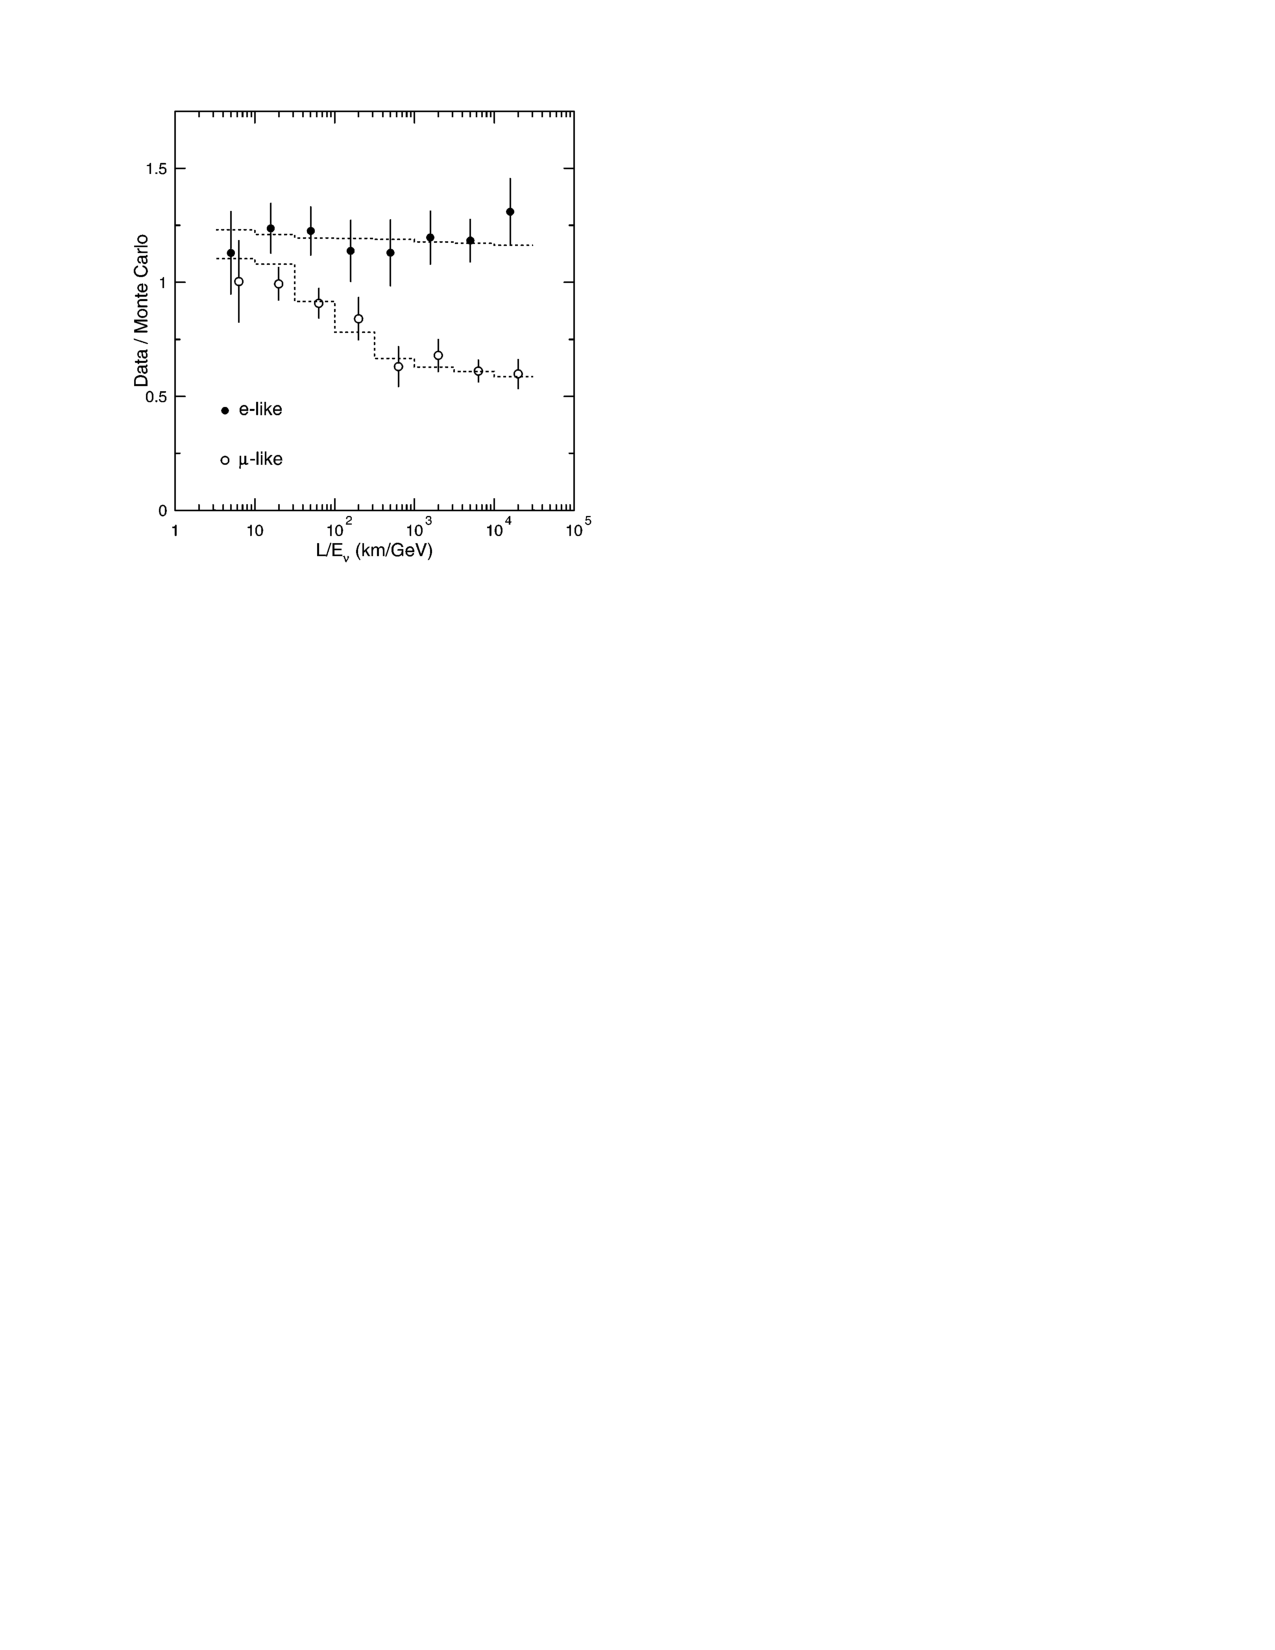
\includegraphics[height=.40\textwidth]{images/NeutrinoPhysics/super_kamiokande}
   \label{fig:super_kamiokande}} \quad
\subfloat[][]
   {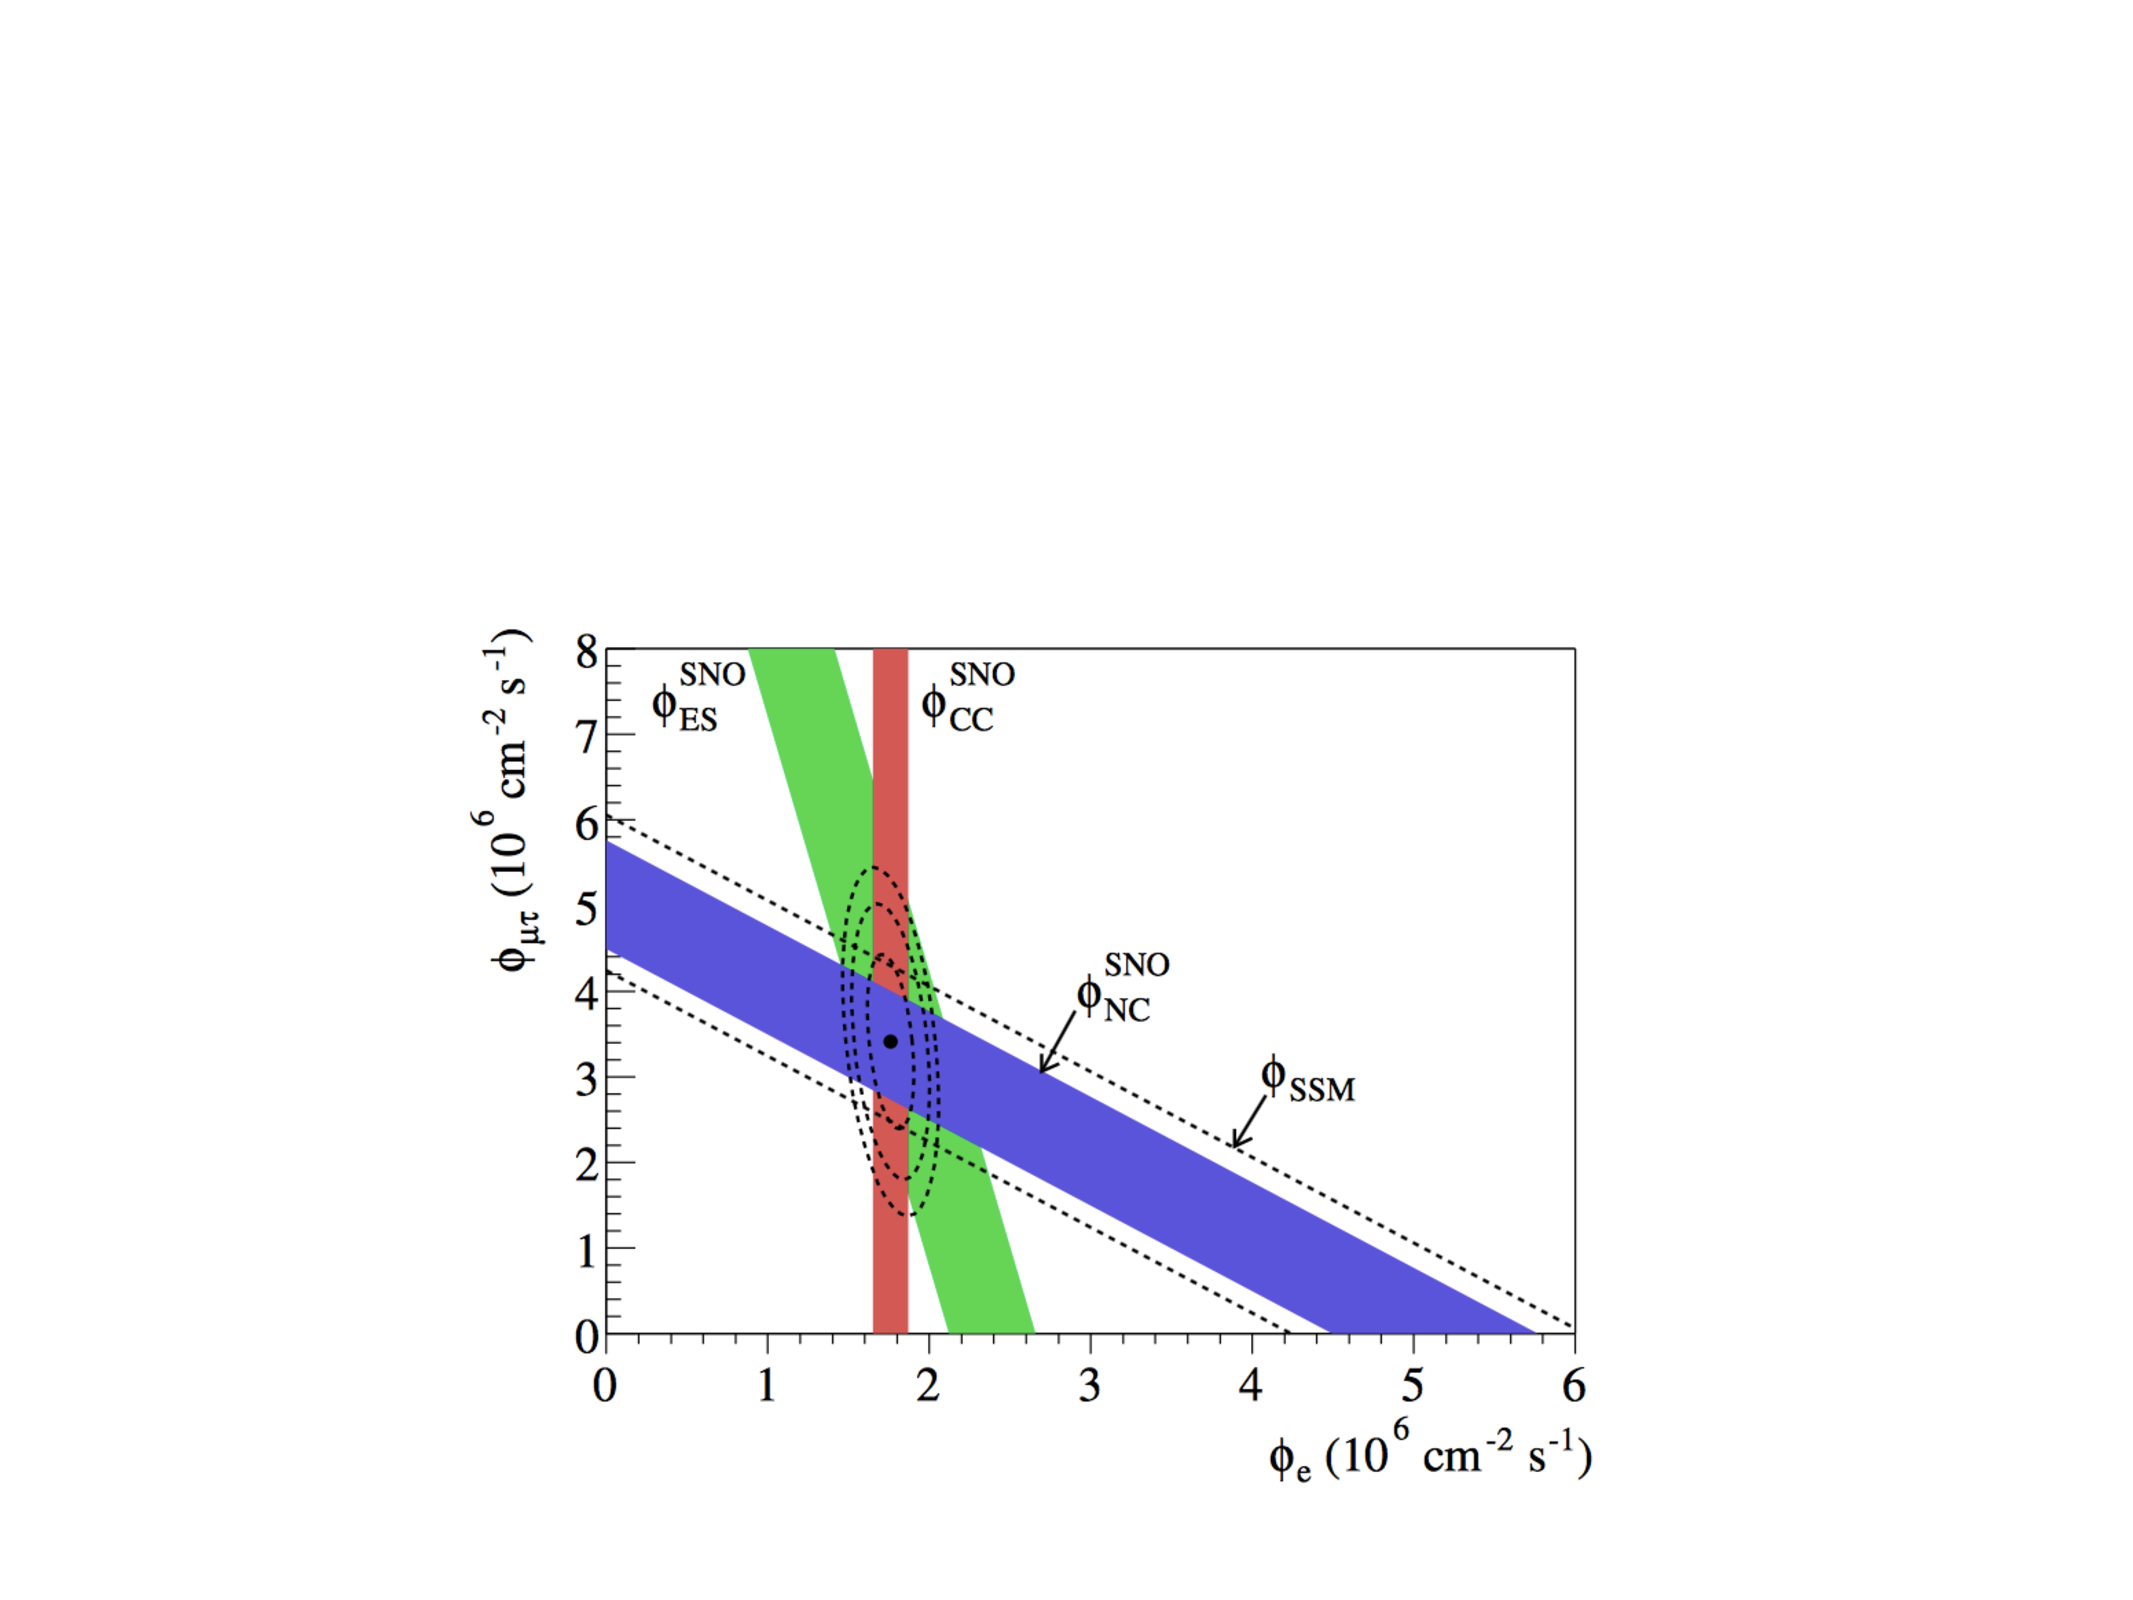
\includegraphics[height=.40\textwidth]{images/NeutrinoPhysics/sno}
   \label{fig:sno}} \\
\caption[Super-Kamiokande and SNO Oscillations]{\protect\subref{fig:super_kamiokande}~The ratio of number of data events to predicted number of events without neutrino oscillations (from Monte Carlo) as a function of $L/E_\nu$ in Super-Kamiokande. The points show the ratio of data to prediction, and the dashed lines show the expected shape when accounting for $\nu_\mu \rightarrow \nu_\tau$ oscillation. Figure source:~\cite{superk}.
\protect\subref{fig:sno}~The solar neutrino fluxes measured by SNO. The flux of muon plus tau neutrinos v.s. the flux of electron neutrinos is shown. The solid bands show the \acrshort{cc}, \acrshort{nc} and \acrshort{es} flux measurements. The dashed line shows the Solar Standard Model prediction. The best fit point is shown with 68\%, 95\% and 99\% contours. Figure source:~\cite{sno}.}
\label{fig:superk_sno}
\end{figure}

In 2002, the Sudbury Neutrino Observatory (SNO) experiment made precise measurements of solar neutrinos. SNO is a heavy water Cherenkov detector in a nickel mine in Ontario (Canada) at a depth of 204 m of rock. The detector contained 1000 tons of $D_2O$~\cite{sno}. This experiment measured the electron and non-electron component of the solar neutrino spectrum by comparing the \acrfull{cc}, \acrfull{nc} and \acrfull{es} neutrino reactions on deuterium. 
%The result from this experiment was a detailed confirmation of the flavour changing signature of neutrino oscillation.
The result from this experiment was a detailed confirmation of the flavour changing signature of solar neutrinos, although this is explained by adiabatic flavour conversion of neutrinos in the matter of the Sun and not by neutrino oscillations~\cite{Smirnov:2016xzf}.
Figure~\ref{fig:superk_sno} shows the allowed fluxes determined by the \acrshort{cc}, \acrshort{nc} and \acrshort{es} measurements. The intersection of the three bands allows resolution of the fluxes of the muon and tau neutrinos and shows the consistency of the three measurements.
%
No $L/E_\nu$ dependence was observed in SNO and mechanism of the neutrino transformation was  not identified. After the SNO results, a number of solutions of the solar neutrino problem still existed~\cite{Smirnov:2016xzf}: matter effects conversion (see Section~\ref{sec:neutrino_oscillations_matter}), resonant spin-flavour precession, Lorentz symmetry violation, decoherence, neutrino decay, and others.

In 2002, KamLAND selected the unique solution of the solar neutrino problem and showed that non-zero neutrino mass is behind the SNO result. The KamLAND experiment found the first evidence for reactor $\bar{\nu}_e$ oscillations. The experiment consists in a liquid scintillator anti-neutrino detector that measured the $\bar{\nu}_e$ flux from nuclear reactors at an average distance of 180 km~\cite{kamland}. 
This experiment observed $258$ events with an expected $365 \pm 24$ events for the case of no oscillations. The $L/E_\nu$ dependence of the survival probability has also been observed. 

In 2010, the observation of a $\nu_\tau$ particle in a $\nu_\mu$ beam was announced by the OPERA experiment~\cite{OPERA}. The OPERA experiment has been designed to search for $\nu_\mu \rightarrow \nu_\tau$ oscillations in appearance mode through the detection of the $\tau$-lepton produced in the $\nu_\tau$ \acrshort{cc} interactions. The detector is located at Gran Sasso, 730 km away from the source in Geneva. \\




No experiments that have been performed so far have detected conclusive deviations from the \acrshort{sm}, except neutrino oscillation experiments, which have shown that neutrinos are massive. In the \acrshort{sm}, this is not the case. This discovery has confirmed that the \acrshort{sm} in an effective theory of the yet unknown theory beyond the \acrshort{sm}. 
%The understanding of how the neutrinos would gain tiny masses and how they are mixed is an extremely challenging task to face. The answer must be found in a theory beyond the SM. Thus, the neutrino is playing the role of a messenger of the new physics beyond the SM.


The phenomenon of neutrino oscillation has been observed for neutrinos from many sources, the sun, reactors, \acrfull{cr} interactions, and accelerator beams~\cite{pdg}. While these experiments provide information about neutrino mixing angles and differences in the square of their masses, complete knowledge of neutrinos is still missing. Remaining questions are mainly the absolute mass of neutrinos (since oscillations are only sensitive to the difference of the square of the masses), whether there is \acrshort{cp} violation in the neutrino sector, the neutrino mass ordering and if they are Dirac ($\nu \neq \bar{\nu}$) or Majorana ($\nu = \bar{\nu}$) particles.



















\section{Neutrino Oscillations}
\label{sec:neutrino_oscillations_vacuum}

%Although the first evidence dates 1968, the concept of neutrino oscillations was first proposed in 1957 by Pontecorvo \cite{pontecorvo}, in analogy with the $K^0-\bar{K}^0$ oscillation phenomenon (M. Gell-Mann and A. Pais), in which the strangeness quantum number is oscillating. 
Neutrino oscillations are generated by the interference of different massive neutrinos, which are produced and detected coherently because of their very small mass differences. 
%The theory of neutrino oscillations was finally settled in 1975-76 by S. Eliezer and A.R. Swift, H. Fritzsch and P. Minkowski, S.M. Bilenky and B. Pontecorvo  as main contributors.\\

Neutrinos $\nu_\alpha$ with flavour $\alpha = e$, $\mu$, $\tau$ are produced in particle decay or in \acrshort{cc} weak interactions processes. Neutrinos of any flavour can also be produced in the \acrshort{nc} weak interaction process $Z \rightarrow \nu\bar{\nu}$. The \acrshort{cc} processes are generated by the \acrshort{cc} leptonic interaction Lagrangian \cite{halzen}:
\begin{equation}
\label{eqn:lagrangian}
\mathscr{L} = -\frac{g}{2\sqrt{2}}\left( J^\rho W_\rho + {J^\rho}^\dagger W_\rho^\dagger \right).
\end{equation}
where $g$ is the coupling constant, $W_\rho$ is the $W$ boson field and $J^\rho$ is the leptonic \acrshort{cc}:
\begin{equation}
J^\rho = 2 \sum_{\alpha=e,\mu,\tau} \sum_k U^*_{\alpha k} \bar{\nu}_k \gamma^\rho l_\alpha.
\end{equation}
The leptonic current $J^\rho$ in Equation~\eqref{eqn:lagrangian} generates a superposition of massive neutrinos whenever the energies and momenta of the particles involved in the neutrino production process are not measured with a degree of accuracy allowing the determination, through energy-momentum conservation, of the emitted massive neutrino. This is the case for neutrino oscillations, in which a flavour neutrino $\nu_\alpha$ is a superposition of massive neutrinos $\nu_k$ with weights proportional to $U^*_{\alpha k}$. 




%\section{Neutrino oscillations in vacuum}

Let us consider a neutrino with flavour $\alpha$ and momentum $\mathbf{p}$, produced in a \acrshort{cc} weak interaction from a charged lepton $l_\alpha$.
In the standard theory of neutrino oscillations, the neutrino flavour state is described by:
\begin{equation}
\label{eqn:mix}
\ket{\nu_\alpha} = \sum_k U^*_{\alpha k} \ket{\nu_k},
\end{equation}
where $U$ is the unitary mixing matrix, called PMNS (Pontecorvo, Maki, Nakagawa and Sakata) matrix.
In the case of three mass eigenstates and three flavour eigenstates, $U$ takes the form:
\begin{equation}
U
=
\begin{pmatrix}
U_{e1} & U_{e2} & U_{e3} \\ 
U_{\mu 1} & U_{\mu 2} & U_{\mu 3} \\ 
U_{\tau 1} & U_{\tau 2} & U_{\tau 3}
\end{pmatrix}.
\end{equation}
The $3 \times 3$ PMNS matrix can be parameterised in terms of three mixing angles $\theta_{12}$, $\theta_{13}$, and $\theta_{23}$ and three \acrshort{cp}-violating phases $\delta_\text{\acrshort{cp}}$, $\alpha_1$, and $\alpha_2$:
\begin{equation}
\label{eq:pmns}
U
=
\underbrace{
\begin{pmatrix}
1 & 0 & 0 \\ 
0 & c_{23} & s_{23} \\ 
0 & -s_{23} & c_{23} 
\end{pmatrix}
}_\text{Atmospheric}
\underbrace{
\begin{pmatrix}
c_{13} & 0 & s_{13}e^{-i\delta_\text{\acrshort{cp}}} \\ 
0 & 1 & 0 \\ 
-s_{13}e^{i\delta_\text{\acrshort{cp}}} & 0 & c_{13} 
\end{pmatrix}
}_\text{Cross-mixing}
\underbrace{
\begin{pmatrix}
c_{12} & s_{12} & 0 \\ 
-s_{12} & c_{12} & 0 \\ 
0 & 0 & 1 
\end{pmatrix}
}_\text{Solar}
\underbrace{
\begin{pmatrix}
e^{i\frac{\alpha_1}{2}} & 0 & 0 \\ 
0 & e^{i\frac{\alpha_2}{2}}  & 0 \\ 
0 & 0 & 1
\end{pmatrix}
}_\text{Majorana}.
\end{equation}
$U$ has been decomposed into four component matrices in Equation~\eqref{eq:pmns} to make it easier to read and interpret, and because different mixing angles are measured by different types of experiment. The first matrix includes only the mixing angle $\theta_{23}$. The third matrix includes only the mixing angle $\theta_{12}$, which dominates the mixing of solar neutrinos.
The second matrix is known as the cross-mixing matrix, and depends on two parameters: the mixing angle $\theta_{13}$ and the \acrshort{cp}-violating phase $\delta_\text{\acrshort{cp}}$. A non-zero $\delta_\text{\acrshort{cp}}$ will lead to a complex matrix $U$ and different probabilities for the \acrshort{cp}-conjugate oscillations $P(\nu_\alpha \rightarrow \nu_\beta) \neq P(\bar{\nu}_\alpha \rightarrow \bar{\nu}_\beta)$, which would be a significant finding. 

The final matrix in Equation~\eqref{eq:pmns} contains the so-called ``Majorana'' \acrshort{cp}-violating phases. These lead to physical effects only for the case of Majorana neutrinos (i.e. where neutrinos are their own antiparticle) and do not conserve lepton number.
Even in the case of Majorana neutrinos, these \acrshort{cp}-violating phases do not affect the oscillation probability, which (as in Equation~\eqref{eqn:prob1}) depends on $\sum_i U^*_{\alpha i} U_{\alpha j}$, so the Majorana phases cancel. It is not possible to determine whether neutrinos are their own antiparticles from oscillation measurements; other experiments (such as the search for neutrinoless double beta decay being conducted or planned by the MAJORANA~\cite{majorana}, GERDA~\cite{gerda}, CUORE~\cite{cuore}, SNO+~\cite{sno_betabeta}, NEXT~\cite{next} and nEXO~\cite{nexo} collaborations, among others) are needed to answer this question. If the neutrinos are instead different from anti-neutrinos, they are ``Dirac'' particles and acquire their mass in a similar way as other fermions in the \acrshort{sm} do.\\





Considering orthonormal massive neutrino states ($\braket{\nu_k|\nu_j} = \delta_{kj}$), the unitary of the mixing matrix implies that also the flavour states are orthonormal: $\braket{\nu_\alpha|\nu_\beta} = \delta_{\alpha\beta}$. Since the massive neutrino states $\nu_k$ are eigenstates of the Hamiltonian, $\mathscr{H} \ket{\nu_k} = E_k\ket{\nu_k}$, with energy 
\begin{equation}
\label{eqn:energy}
E_k = \sqrt{\mathbf{p}^2+m_k^2},
\end{equation}
 then the Schrodinger equation
\begin{equation}
i\frac{d}{dt}\ket{\nu_k(t)} = \mathscr{H} \ket{\nu_k(t)},
\end{equation}
implies that the massive neutrino states evolve in time as plane waves:
\begin{equation}
\label{eqn:plane_wave}
\ket{\nu_k(t)} = e^{-iE_k t}\ket{\nu_k}.
\end{equation}
Considering now a flavour state $\ket{\nu_\alpha(t)}$ which describes a neutrino created with a definite flavour $\alpha$ at time $t=0$. From Equations~\eqref{eqn:mix} and \eqref{eqn:plane_wave}, the time evolution of this state is given by
\begin{equation}
\label{eqn:mix2}
\ket{\nu_\alpha(t)} = \sum_k U^*_{\alpha k} e^{-iE_k t} \ket{\nu_k},
\end{equation}
such that
\[
\ket{\nu_\alpha(0)} =\ket{\nu_\alpha}.
\]
The massive states can be expressed in terms of flavour states inverting Equation~\eqref{eqn:mix}:
\begin{equation}
\ket{\nu_k} = \sum_\alpha U_{\alpha k} \ket{\nu_\alpha},
\end{equation}
where the relation $U^\dagger U = \mathbf{1}$ has been used. Substituting the last relation into Equation \eqref{eqn:mix2} one gets:
\begin{equation}
\label{eqn:mix3}
\ket{\nu_\alpha (t)} = \sum_{\beta=e,\mu,\tau} \left ( \sum_k U^*_{\alpha k} e^{-i E_k t} U_{\beta k} \right ) \ket{\nu_\beta}.
\end{equation}
Hence, the superposition of massive neutrino states $\ket{\nu_\alpha (t)}$, and the pure flavour state given in Equation~\eqref{eqn:mix} at $t = 0$, becomes a superposition of different flavour states at $t > 0$. 
%As it turns out the mixing matrix $U$ is not diagonal: neutrinos are mixed. 
The transition probability of $\ket{\nu_\alpha} \rightarrow \ket{\nu_\beta}$ as a function of time is given by:
\begin{equation}
P_{{\nu_\alpha} \rightarrow {\nu_\beta}} (t) = | \braket{\nu_\beta | \nu_\alpha} |^2 = \sum_{k,j} U^*_{\alpha k}U_{\beta k} U_{\alpha j} U^*_{\beta j} e^{-i (E_k-E_j)t}.
\end{equation}
For ultra-relativistic neutrinos, one could expand Equation \eqref{eqn:energy} considering $m_k \sim 0$ to obtain $E_k \simeq E + {m_k^2}/{2E}$, where $E=|\mathbf{p}|$. Given the mass difference $\Delta m_{kj}^2$ it is possible to write:
\begin{equation}
E_k-E_j\simeq \frac{\Delta m_{kj}^2}{2E}.
\end{equation}
In neutrino oscillation experiments, the propagation time $t$ is not measured. What is known is the distance $L$ between the source and the detector. Since ultra-relativistic neutrinos propagate almost at the speed of light, it is possible to approximate $t = L$. Therefore, the transition probability can be approximated by:
\begin{equation}
\label{eqn:prob1}
P_{{\nu_\alpha} \rightarrow {\nu_\beta}} (t) = \sum_{k,j} U^*_{\alpha k}U_{\beta k} U_{\alpha j} U^*_{\beta j} e^{-i \frac{\Delta m_{kj}^2 L}{2E}}.
\end{equation}

The oscillation probability thus depends both on quantities fixed by nature (PMNS matrix elements and differences of the square of the masses $\Delta m^2$) and on parameters fixed by experiments (the path the neutrino travels $L$, i.e. the source-detector distance, and the neutrino energy $E$).
Moreover, oscillation experiments are only sensitive to the difference of the squares of the masses and not to the absolute neutrino mass.

The now well-accepted picture of neutrino mixing involves three underlying mass states, with three mixing angles defining the linear superpositions that make up each of the three weak, or flavour, states. The magnitude of the mass-squared splitting between states $\nu_1$ and $\nu_2$ is known from the KamLAND reactor experiment~\cite{kamland}, and the much-larger splitting between the third, $\nu_3$ state and the $\nu_1 - \nu_2$ pair is known from atmospheric and long-baseline experiments~\cite{pdg}. However, pure neutrino oscillations are sensitive only to the magnitude of the mass splitting, not to its sign. Defining the $\nu_1$ state as having the largest admixture of the electron flavour eigenstate, the sign of the mass splitting between states $\nu_2$ and $\nu_1$ is determined to be positive ($\Delta m^2_{21} > 0$) using the pattern of neutrino oscillations through the varying-density solar medium~\cite{pdg}. However, the corresponding sign of $\Delta m^2_{32} \sim \Delta m^2_{31}$ remains unknown. That is, there are two potential orderings, for the neutrino mass states: the so-called \emph{normal ordering}, in which $\nu_3$ is the heaviest, and the \emph{inverted ordering}, in which $\nu_3$ is the lightest, as shown in Figure \ref{fig:hierarchy}.\\

%++++++++++++++++++++
\begin{figure}[]
\centering
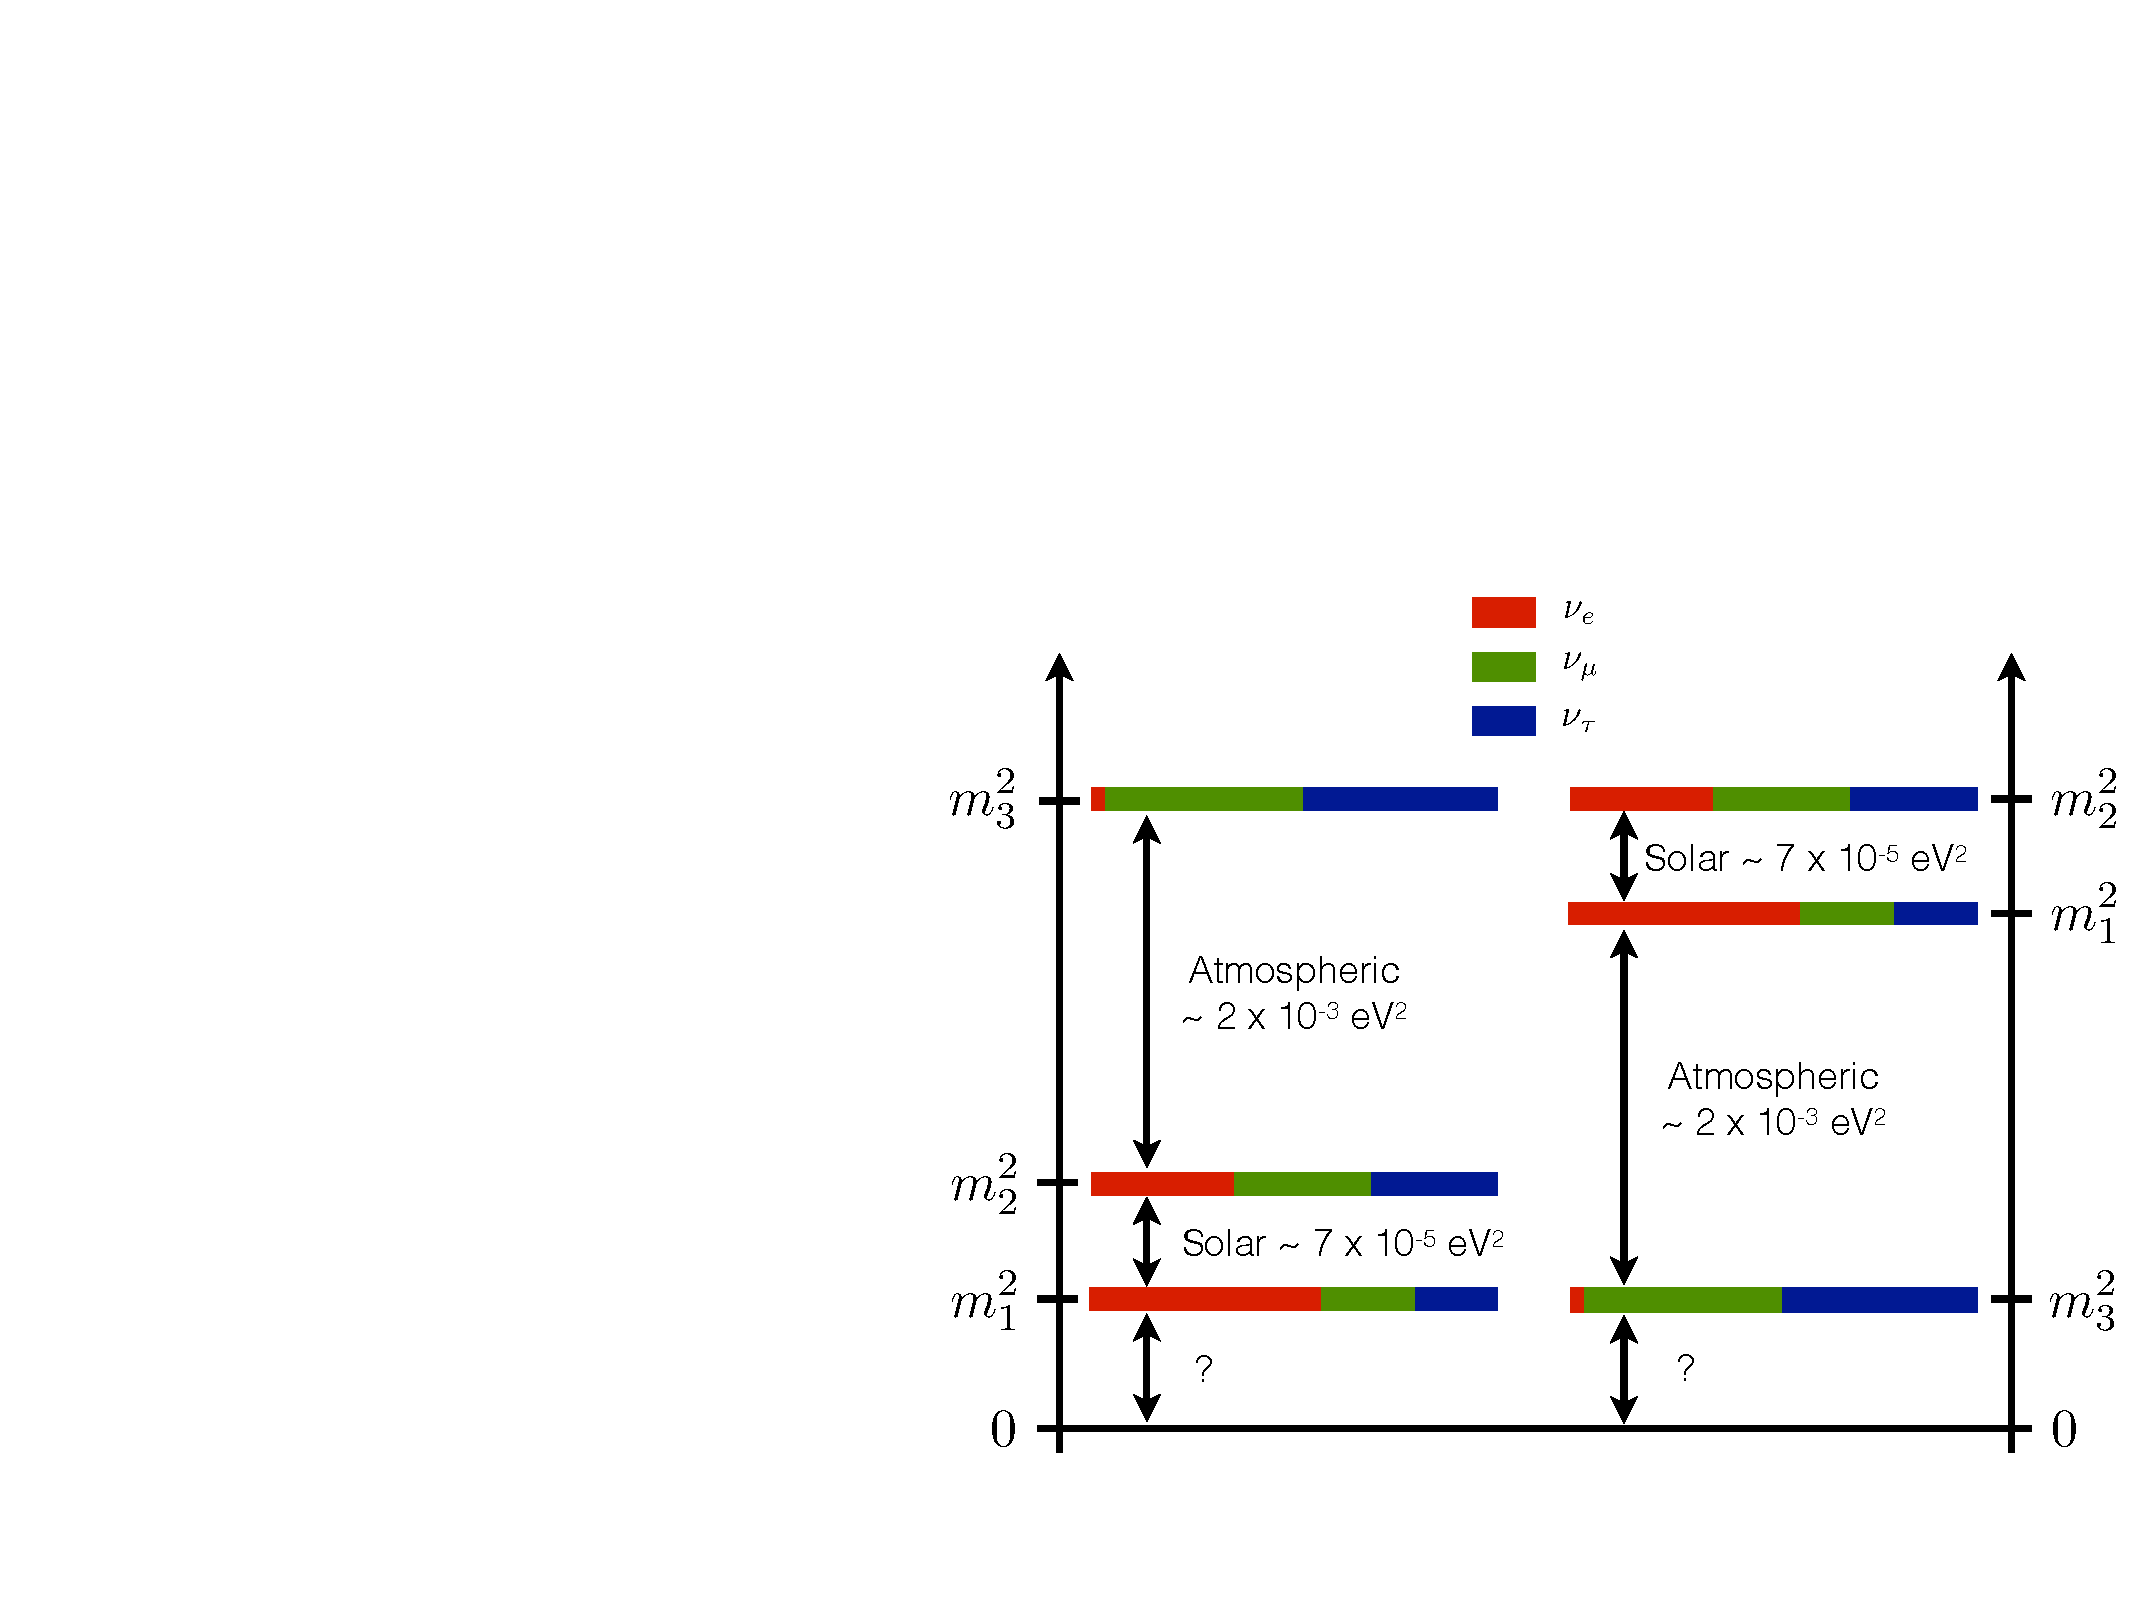
\includegraphics[width=0.7\textwidth]{mass_hierarcy_myPIC}
\caption[Mass Ordering]{Pictorial representation of the possible neutrino mass orderings. Note: $\Delta m^2_\text{atm}$ is equivalent to $\Delta m^2_{32}$ and $\Delta m^2_\text{sol}$ is equivalent to $\Delta m^2_{21}$.}
\captionsetup{format=hang,labelfont={sf,bf}}
\label{fig:hierarchy}
\end{figure}
%++++++++++++++++++++

%The transitions among different flavours manifest for $L > 0$, because the unitarity relation
%\[
%UU^\dagger = \mathbf{1} \qquad\Longleftrightarrow \qquad \sum_k U_{\alpha k} U_{\beta k}^* = \delta_{\alpha \beta},
%\]
%implies that
%\[
%P_{\nu_\alpha \rightarrow_\beta} (L=0,E) = \delta_{\alpha \beta}.
%\]
%It is possible to show that:
%\begin{itemize}
%\item The sum of the probabilities of transition from a flavor neutrino $\nu_\alpha$ to all flavor neutrinos $\nu_\beta$ is equal to unity:
%\[
%\sum_\beta P_{\nu_\alpha \rightarrow \nu_\beta}(L,E) = 1.
%\]
%\item The sum of the probabilities of transition from any flavor neutrino $\nu_\alpha$ to a flavor neutrino $\nu_\alpha$ is equal to unity:
%\[
%\sum_\alpha P_{\nu_\alpha\rightarrow\nu_\beta}(L,E) = 1.
%\]
%\end{itemize}


%\subsection{General remarks}
%\label{sec:GenRem}
%The main assumptions adopted in the standard derivation of the neutrino oscillation probability can be summarized as follows.
%\begin{itemize}
%\item Flavour neutrinos have a definite momentum $\mathbf{p}$, i.e. all the massive neutrino components have the same momentum. This is also called the \emph{equal momentum assumption}. In principle, there is no justification for this assumptions. However, it is possible to see that the equal momentum assumption is irrelevant in the derivation of the oscillation probability.
%\item The propagation time $t$ is equal to the distance $L$ traveled by the neutrino between production and detection. This is called the \emph{light-ray approximation}. This assumption is unjustified in a plane-wave treatment of oscillations, because plane waves extend with the same amplitude over the whole space-time. However, in quantum theory, localized particles are described by wave packets. In fact, neutrinos are described by wave packets that are localized in the production process at the production time and propagate between the production and the detection processes with a group velocity close to the velocity of light, justifying the approximation $t = L$.
%\end{itemize}






%\subsection{PMNS matrix}
%
%In the standard picture of neutrino oscillations with three active neutrino flavours and no sterile states the $3 \times 3$ PMNS matrix is written in the form:
%
%\begin{equation}
%\begin{pmatrix}
%\ket{\nu_e} \\ \ket{\nu_\mu} \\ \ket{\nu_\tau}
%\end{pmatrix}
%=
%\begin{pmatrix}
%U_{e1} & U_{e2} & U_{e3} \\ 
%U_{\mu 1} & U_{\mu 2} & U_{\mu 3} \\ 
%U_{\tau 1} & U_{\tau 2} & U_{\tau 3}
%\end{pmatrix}
%\begin{pmatrix}
%\ket{\nu_1} \\ \ket{\nu_2} \\ \ket{\nu_3}
%\end{pmatrix}
%\end{equation}
%
%The standard parametrization of PMNS mixing matrix in terms of three mixing angles and a \acrshort{cp}-violating phase is given as follows:
%\begin{equation}
%\begin{split}
%U_{e2} &= \cos\theta_{13}\sin\theta_{12}          \\
%U_{\mu 3} &= \cos\theta_{13}\sin\theta_{23}       \\
%U_{e3} &= \sin\theta_{13}e^{-i\delta_\text{\acrshort{cp}}}   \\
%\end{split}
%\end{equation}
%with all other elements following by unitarity. The square of the elements of the PMNS matrix give the fractional flavor content, e.g. $|U_{e2}|^2$ is the fraction of $\nu_2$ that is $\nu_e$. Figure \ref{fig:hierarchy} gives this fraction for all the mass eigenstates.







%Alternatively, it is possible to write:
%\begin{equation}
%\sin^2\theta_{13} = |U_{e3}|^2, \quad \sin^2\theta_{12} = \frac{|U_{e2}|^2}{(1-|U_{e3}|^2)} \sim |U_{e2}|^2, \quad  \sin^2\theta_{23} =\frac{|U_{\mu 3}|^2}{(1-|U_{e3}|^2)} \sim |U_{\mu 3}|^2,
%\end{equation}
%where the $\sim$ follows from the fact that  $|U_{e3}|^2 \ll 1$ \footnote{Day Bay reactor experiment measured $\sin^22\theta_{13} = 0.084 \pm 0.005$, \cite{daya}.}.
%
%
%
%At the end one can write the PMNS matrix as follows:
%\begin{center}
%\begin{equation}
%U
%=
%\begin{pmatrix}
%c_{12}c_{13} &s_{12}c_{13} & s_{13}e^{-i\delta_\text{\acrshort{cp}}} \\ 
%-s_{12}c_{23}-c_{12}s_{23}s_{13}c_{12}s_{23} & c_{12}c_{23}-s_{12}s_{23}s_{13}e^{i\delta_\text{\acrshort{cp}}} & s_{23}c_{13} \\ 
%s_{12}c_{23}-c_{12}c_{23} s_{13}e^{-i\delta_\text{\acrshort{cp}}} & -c_{12}s_{23}-s_{12}c_{23}s_{13}e^{i\delta_\text{\acrshort{cp}}}& c_{23}c_{13}
%\end{pmatrix}
%\end{equation}
%\end{center}
%where $c_{ij} \equiv \cos\theta_{ij}$ and $s_{ij} \equiv \sin\theta_{ij}$. This matrix depends on: three mixing angles $\theta_{12}$, $\theta_{13}$, and $\theta_{23}$, of which the first and last are the dominant angles for solar and atmospheric oscillations, respectively; a Dirac phase $\delta_\text{\acrshort{cp}}$ that can induce \acrshort{cp}-violating differences in the oscillation probabilities for conjugate channels such as $\nu_\mu \rightarrow \nu_e$ versus $\bar{\nu}_\mu \rightarrow \bar{\nu}_e$.
%



\section{Neutrino Oscillations In Matter}
\label{sec:neutrino_oscillations_matter}


Neutrinos propagating in matter are subject to a potential due to the coherent forward elastic scattering with the particles in the medium (electrons and nucleons). Coherent scattering happens when the neutrino wave function interacts with the matter as a whole, such as the scattered waves from the nuclei in the matter interfere with each other.


%Neutrinos in matter are also affected by \emph{incoherent} scattering with particles in the medium. In an incoherent scattering, the neutrino wave function scatters with each single nucleus independently in such a way that the scattered waves do not interfere, but they sum up incoherently. However, as shown below, this contribution can be neglected for artificial terrestrial neutrino sources.
%
%Let us consider the cross section of a neutrino weakly interacting with a lepton or a hadron. From dimensional arguments, in the center of mass frame we get
%\begin{equation}
%\sigma \sim G_F\,s
%\end{equation}
%where $s$ is the Lorentz invariant Mandelstam variable which represent the squared center of mass energy and $G_F$ is the Fermi constant: $G_F = 1.16\times10^{-5}GeV^{-2}$. Being $s$ invariant, we can express it in the laboratory frame neglecting the neutrino mass. We get: $s=2EM$, where $E$ is the neutrino energy and $M$ the mass of the lepton or the hadron. This yields:
%\begin{equation}
%\sigma \sim G_F\,E\,M \sim 10^{-38} \text{cm}^2 \,\frac{E\,M}{\text{GeV}^2}
%\end{equation}
%We can now evaluate the mean free path $\lambda$ of a neutrino traversing a medium with number density $N$ of target particles:
%\begin{equation}
%\lambda \sim \frac{1}{N\,\sigma} \sim \frac{10^{38} \text{cm}^2}{(N\, \text{cm}^3)\,(E\,M/ \text{GeV}^2)}
%\end{equation}
%For neutrinos traversing the Earth's crust, the main target particles are nucleons with mass $M\sim 1$ GeV and number density $N \sim N_A/\text{cm}^3 \sim 10^{24}/\text{cm}^3$. So that:
% \begin{equation}
%\lambda_{\text{Earth}} \sim \frac{10^{14}\,\text{cm}}{(E/\text{Gev})}
%\end{equation}
%If we take for example the NO$\nu$A experiment, the neutrino energy is about $2$ GeV. This yields $\lambda_{\text{Earth}} \sim 10^{14}$ cm. Considering that the Earth diameter is about $10^9$ cm, we can conclude that the Earth is nearly transparent for neutrinos. Hence the contribution of incoherent scattering can be neglected. \\

When active flavour neutrinos propagate in matter, their evolution equation is affected by both \acrshort{cc} and \acrshort{nc} scatterings \cite{giunti}.  The Feynman diagrams of \acrshort{cc} and \acrshort{nc} scattering are shown in Figure \ref{fig:diagram}. This phenomenon was first proposed by Wolfenstein \cite{wolfenstein} and is now known as the \acrfull{msw} effect.

%mpost fgraphs
%mpost fgraphs2
%+++++++++FIGURE+++++++++
\begin{figure}[]
\centering
\subfloat[][]
   {
   \centering
   \begin{fmffile}{fgraphs}
     \begin{fmfgraph*}(40,38)
       % Define two vertices on the left, but only `i2' will be actually used.
       \fmfleft{i1,i2}
       % The same on the right.
       \fmfright{o1,o2}
       % Define the vertex for the blob.
       \fmfbottom{b}
       \fmf{fermion}{i2,v2}
       \fmf{fermion}{v2,o2}
       \fmf{photon, label=$W$, label.side=left}{v2,v1} 
       \fmf{fermion}{i1,v1}
       \fmf{fermion}{v1,o1}
       % Labels on vertices.
       \fmflabel{$\nu_e$}{i2} \fmflabel{$e^-$}{o2}
       \fmflabel{$e^-$}{i1} \fmflabel{$\nu_e$}{o1}
     \end{fmfgraph*}
   \end{fmffile}
   \label{fig:diagram1}  
   } \qquad\qquad \qquad
   \subfloat[][]
   {
   \centering
   \begin{fmffile}{fgraphs2}
     \begin{fmfgraph*}(40,38)
       % Define two vertices on the left, but only `i2' will be actually used.
       \fmfleft{i1,i2}
       % The same on the right.
       \fmfright{o1,o2}
       % Define the vertex for the blob.
       \fmfbottom{b}
       \fmf{fermion}{i2,v2}
       \fmf{fermion}{v2,o2}
       \fmf{photon, label=$Z$, label.side=left}{v2,v1} 
       \fmf{fermion}{i1,v1}
       \fmf{fermion}{v1,o1}
       % Labels on vertices.
       \fmflabel{$\nu_e$, $\nu_\mu$, $\nu_\tau$}{i2} \fmflabel{$\nu_e$, $\nu_\mu$, $\nu_\tau$}{o2}
       \fmflabel{$e^-$, $p$, $n$}{i1} \fmflabel{$e^-$, $p$, $n$}{o1}
     \end{fmfgraph*}
   \end{fmffile}
   \label{fig:diagram2}
   } \\
\caption[Feynman Diagrams for Coherent Electron Neutrino Scattering]{Feynman diagrams of the coherent forward elastic scattering processes.}
\label{fig:diagram}
\end{figure}
%++++++++++++++++++++++++

A full account of how exactly these matter effects alter neutrino oscillation probabilities is beyond the scope of this thesis (although it is well described in other sources, e.g.~\cite{giunti}).

An important implication of matter effects in neutrino oscillations is that their impact is different for neutrinos and antineutrinos (since the \acrshort{cc} interaction shown in Figure~\ref{fig:diagram1} is not available for antineutrinos) due to the lack of positrons in the Earth. This can mimic a \acrshort{cp} violation $P(\nu_\alpha \rightarrow \nu_\beta) \neq P(\bar{\nu}_\alpha \rightarrow \bar{\nu}_\beta)$ effect which does not say anything interesting about matter-antimatter asymmetry at a fundamental level. It is therefore essential to account for matter effects when attempting to determine $\delta_\text{\acrshort{cp}}$ to identify genuine neutrino-sector \acrshort{cp} violation.

Moreover, whilst vacuum oscillations are only sensitive to the square of the neutrino mass splitting, matter effects are sensitive to the signs of the mass splittings. 
Current and future experiment will have sensitivity to a mass ordering measurement.
%Exploiting this in solar neutrino observations has allowed the determination that $\nu_2$ is greater than $\nu_1$, but it is not yet known whether $\nu_3$ is the heaviest (a `normal neutrino mass ordering`) or the lightest (an `inverted neutrino mass ordering`).
%As the baseline itself is a critical factor for sensitivity, experiments are classified either as near and relatively long baseline (like T2K \cite{T2K} and NO$\nu$A \cite{patterson}), or as very long baseline experiments (DUNE, \cite{DUNE}). 
While T2K~\cite{t2k_systs} has very little sensitivity to the ordering, due to the shorter baseline, NO$\nu$A~\cite{patterson} has the potential to make a measurement at the $2-3\sigma$ level, if the value of the \acrshort{cp} phase parameter $\delta_\text{\acrshort{cp}}$ is maximal.
A combination of current experiments at different baselines (e.g. T2K+NO$\nu$A) could help to further disentangle the competing effects of \acrshort{cp} violation and matter-induced neutrino-anti-neutrino differences. However, the future DUNE~\cite{DUNE} experiment will identify the mass ordering, removing the ambiguities.  \\

There are several motivations as to why to determine the neutrino mass ordering. Once the ordering is understood, the uncertainty on a measurement of the \acrshort{cp}-violating phase, $\delta_\text{CP}$, is significantly reduced. Knowledge of the mass ordering would define the scope for future neutrinoless double beta decay experiments, seeking to resolve the mass nature of the neutrino, by limiting the domain for observation of a signal. In combination with cosmological measurements, which are sensitive to the sum of neutrino masses, knowledge of the mass ordering could also be used to determine the absolute mass scale of neutrinos. Furthermore, it will allow constraining many of the grand unification theories~\cite{pdg} and will help in the understanding of core-collapse supernovae. 
For these many reasons, determination of the neutrino mass ordering is thus a fundamental step towards completion of the \acrshort{sm} of particle physics.





\section{Overview of Neutrino Oscillation Experiments}
\label{sec:neutrino_oscillations_experiments}

%In general,  neutrino oscillation experiments are classified into appearance experiments (which measure transitions between different neutrino flavours, i.e. they look for the oscillation of $\nu_\alpha \rightarrow \nu_\beta$ measuring $\nu_\beta$) and disappearance experiment (which measure the survival probability of a neutrino flavour by counting the number of tagged interactions in the detector and comparing it with the expected one).

Neutrino oscillation experiments are classified based on the different sources of neutrinos that have been used. 
%Natural sources, like solar or atmospheric neutrinos, are not enough to explore all the neutrino oscillation parameters.
\begin{description}
\item[Reactor Neutrino Experiments] These experiments exploit the large isotropic fluxes of electron anti-neutrinos produced in nuclear reactors by $\beta$ decays of heavy nuclei (mainly fission fragments of $^{235}$U, $^{238}$U, $^{239}$Pu, $^{241}$Pu). Typical energy of reactor $\nu_e$'s is of the order of a few MeV. 
%Experiments of this type which have been performed in the past are: KamLAND \cite{kamland},CHOOZ \cite{CHOOZ}, Palo Verde \cite{PALOVERDE}, Daya Bay \cite.
\item[Atmospheric Neutrino Experiments] Primary \acrshort{cr} interact with the upper layers of the atmosphere producing a large flux of pions and kaons which decay in the atmosphere into muons and muon neutrinos. Many muons further decay into electrons and muon neutrinos before hitting the ground. Atmospheric neutrino experiments are designed to detect these $\nu_\mu$. The energy of detectable atmospheric neutrinos covers a very wide range, from about 500 MeV to about 100 GeV, and even higher are possible in a large detector like IceCube~\cite{icecube}. The source-detector distance ranges from about $20$ km for neutrinos coming from above, to about $10^4$ km for neutrinos coming from below, initially produced on the other side of the Earth. Atmospheric neutrino experiments are sensitive to $\Delta m^2$ of the order of $10^{-3} \, \text{eV}^2$ and the current best measurement is $\Delta m^2_{32} = 2.56^{+0.13}_{-0.11} \times 10^{-3}\, \text{eV}^2$~\cite{pdg}, as previously shown in Figure~\ref{fig:hierarchy}.
%Some atmospheric neutrino experiments which have been performed in the past are: Kamiokande \cite{Kamiokande}, Super-Kamiokande \cite{SuperKamiokande}, MACRO \cite{Macro}.
\item[Solar Neutrino Experiments] These experiments detect the electron neutrinos generated in the core of the Sun by the thermonuclear reactions that power the Sun. Solar neutrino experiments are designed to detect these $\nu_e$ and are sensitive to extremely small values of $\Delta m^2$ ($\Delta m^2_{21} = 7.37^{+0.59}_{-0.44} \times 10^{-5}\, \text{eV}^2$~\cite{pdg}), much smaller than the sensitivity of the other experiment discussed above. 
%Several solar neutrino experiments have been performed in the past, like Kamiokande \cite{Kamiokande2} and SNO \cite{SNO}.
\item[Accelerator Experiments] These experiments make use of beams of muon neutrinos produced by the decay of pions, kaons, and muons created by a proton beam hitting a target. They are further classified into \emph{appearance} experiments if they look at electron neutrinos oscillated from the initial muon neutrinos, or \emph{disappearance} experiments if they look at the reduction in muon neutrino events due to oscillations. These experiments are the focus of this thesis and will be better described in the next section. \\
\end{description}

Since the value of $\Delta m^2$ is fixed by nature, different experiments can be designed to be sensitive to different values of $\Delta m^2$, by choosing appropriate values of the ratio $L/E$. From Equation~\eqref{eqn:prob1}, the value of $\Delta m^2$ for which
\[
\frac{\Delta m^2 L}{2E} \simeq 1
\]
is called the sensitivity to $\Delta m^2$ of an experiment.
Different types of neutrino oscillation experiments are then classified depending on the average value of the ratio $L/E$. Short baseline experiments (${L}/{E} \lesssim 1\, \text{km}/\text{GeV}$) are sensitive to $\Delta m^2 \gtrsim 1 \, \text{eV}^2$. Some experiments of this type which have been performed in the past are
BEBC \cite{BEBC}, CDHSW \cite{CDHSW}, CHARM \cite{CHARM}, CHORUS \cite{CHORUS}, NOMAD \cite{NOMAD}, LSND \cite{LSND} and MiniBooNE \cite{miniboone}. 
Long baseline experiment ($\frac{L}{E} \lesssim 10^3\, \text{km}/\text{GeV}$) are sensitive to $\Delta m^2 \gtrsim 10^{-3}$. Some experiments of this type which have been performed in the past and in the present are ICARUS \cite{ICARUS}, OPERA \cite{OPERA}, T2K \cite{t2k_systs}, MINOS \cite{MINOS} and NO$\nu$A \cite{nova}.
%Finally, very long baseline experiment ($\frac{L}{E} \lesssim 10^4\, \text{km}/\text{GeV}$) are sensitive to $\Delta m^2 \gtrsim 10^{-4}$. DUNE \cite{dune} will be a future very long baseline experiment.




%Considering only accelerator neutrino beam, it is then possible to categorise them into:
%\begin{description}
%\item[Short Base-line experiments] The range of $L/E$ covered by these experiments and their sensitivity to  $\Delta m^2$ are:
%\[
%\frac{L}{E} \lesssim 1\, \text{km}/\text{GeV}  \qquad \Longrightarrow \qquad \Delta m^2 \gtrsim 1 \text{eV}^2
%\]
%Some experiments of this type which have been performed in the past are:
%BEBC \cite{BEBC}, CDHSW \cite{CDHSW}, CHARM \cite{CHARM}, CHORUS \cite{CHORUS}, NOMAD \cite{NOMAD}.
%\item[Long Base-line experiments] These are experiments which have sources similar to SBL experiments, but the source-detector distance is about two or three orders of magnitude larger. They measure the atmospheric sector: $\Delta m^2_{32}$. In this case:
%\[
%\frac{L}{E} \lesssim 10^3\, \text{km}/\text{GeV}  \qquad \Longrightarrow \qquad \Delta m^2 \gtrsim 10^{-3}\, \text{eV}^2
%\]
%Some experiments of this type which have been performed in the past and in the present are: ICARUS \cite{ICARUS}, OPERA \cite{OPERA}, T2K \cite{T2K}, MINOS \cite{MINOS} and NO$\nu$A \cite{}.
%\item[Very Long-Baseline experiments] These are accelerator neutrino experiments with a source-detector distance of the order of several thousands of km, comparable with the diameter of the Earth:
%\[
%\frac{L}{E} \lesssim 10^4\, \text{km}/\text{GeV}  \qquad \Longrightarrow \qquad \Delta m^2 \gtrsim 10^{-4}\, \text{eV}^2
%\]
%These experiments are under study; new and more intense neutrino beams are needed in order to observe a sufficient number of events at such large distances.
%
%\end{description}







\section{Challenges in Neutrino Oscillation Experiments}
\label{sec:neutrino_oscillations_challenges}

Accelerator long-baseline neutrino experiments can measure muon neutrino disappearance (and are particularly sensitive to the oscillation parameters $\theta_{23}$ and $\Delta m^2_{23}$) and electron neutrino appearance (are sensitive to the oscillation parameters $\theta_{13}$ and $\delta_\text{\acrshort{cp}}$). These experiments consist of a far detector, positioned close to the oscillation maximum, and a near detector, placed just after the neutrino beam production point, to constrain the properties of the neutrino beam and neutrino interactions. 
%More details of the MicroBooNE experiment can be found in Chapter~\ref{}.


Oscillation experiments measure event rates as a function of energy in their detectors. For a $\nu_\alpha \rightarrow \nu_\beta$ oscillation, the event rate in their far detector can be naively computed as
\begin{equation}
\label{eq:evt_fd}
N^{\alpha\rightarrow\beta}_\text{FD} (E_\text{reco}) = \int \phi_\alpha^\text{FD}(E_\text{true})\, P_{\alpha\rightarrow\beta}(E_\text{true}) \sigma_\beta(E_\text{true}) \epsilon_\beta(E_\text{true}) U^\text{FD}(E_\text{true}, E_\text{reco}) dE_\text{true},
\end{equation}
where $N^{\alpha\rightarrow\beta}_\text{FD} (E_\text{reco})$ is the number of events as a function of reconstructed neutrino energy, $\phi_\alpha^\text{FD}(E_\text{true})$ is the neutrino flux of flavour $\alpha$, $P_{\alpha\rightarrow\beta}(E_\text{true})$ is the oscillation probability, $\sigma_\beta(E_\text{true})$ is the cross section for flavour $\beta$, and $U^\text{FD}(E_\text{true}, E_\text{reco})$ is the detector response function, describing how $E_\text{true}$ is reconstructed in $E_\text{reco}$.

Experiments depend upon a model of the neutrino-nucleus interaction to disentangle neutrino event rates in their detectors. It is clear from Equation~\eqref{eq:evt_fd} that in order to reliably measure the neutrino oscillation probability, $P_{\alpha\rightarrow\beta}$, the unoscillated flux, the detector response and neutrino interaction cross sections must be well understood. If any of these components are not well modelled the extracted oscillation parameters may be biased and large uncertainties on these components will limit the sensitivity of the experiment. 


Neutrino oscillation experiments often employ a near detector to measure the unoscillated rate of interactions. Here, the number of events can be naively computed as
\begin{equation}
\label{eq:evt_nd}
N^{\alpha}_\text{ND} (E_\text{reco}) = \int \phi_\alpha^\text{ND}(E_\text{true})\, \sigma_\alpha(E_\text{true}) \epsilon_\alpha(E_\text{true}) U^\text{ND}(E_\text{true}, E_\text{reco}) dE_\text{true},
\end{equation}
and experiments may either fit the near detector data to constrain model parameters, or correct the energy distribution according to the near detector data and then extrapolate to the far detector. These methods allow to reduce systematic uncertainties as the flux, cross section, detector response and efficiency are usually highly correlated.
However, even when near detector data is used in long-baseline experiments, it does not remove all dependence on the cross-section model. Because event rates correspond to a convolution of the flux and cross section, determinations of oscillation parameters rely on the model to relate near and far detector measurements.
In fact, despite the critical role of the near detectors, the near-far cancellation can never be complete for several reasons. 
First of all, the two detectors might employ different target materials, which require the cross-section extrapolation from one material to another. Moreover, the flux at the near detector cannot be the same as the oscillated one at the far detector as Equation~\eqref{eq:evt_fd} contains the unknown oscillation probability $P_{\alpha\rightarrow\beta}$. The fluxes also differ because the near and far detectors are in two different locations: the near detector sees a line source of neutrinos (pion decays take place along the decay pipe, which typically has a length of a few hundred meters), while the far detector essentially sees a point source. This implies that the acceptance of particles is different at the two detectors.

Another way the cross-section model affects an oscillation analysis is through the efficiencies $\epsilon_\alpha(E_\text{true})$ in Equations~\eqref{eq:evt_fd} and~\eqref{eq:evt_nd}. These efficiencies include both the acceptance of the detector and the efficiency of selection cuts applied to select signal and reject background. Although the efficiency should be independent of any interaction model, in practice it is calculated by taking simulated particles from a neutrino simulator, which generates events according to a particular model. See for example Section~\ref{sec:evt_sel_performances} for the efficiency calculated for the analysis presented in this thesis.
The difference between the near and far detectors leads to uncertainties that do not cancel exactly. 



Finally, another challenge for oscillation experiments is the estimation of the neutrino energy as the oscillation probability in Equation~\eqref{eqn:prob1} depends on it. The true neutrino energy is not an observable and what is actually measured is a reconstructed neutrino energy, that must account for unobserved energy deposition, including particles below detection threshold, inactive material, and escaping neutral particles.
In practice, assumptions about these effects are based on the cross-section model. 
The determination of the reconstructed neutrino energy depends on the detector technology used and can be roughly divided into two different methods \cite{nustec}: kinematical and calorimetric.
With the kinematical method, the energy is reconstructed assuming the interaction is \acrshort{cc} \acrfull{qe}, neglecting the unmeasured recoil momentum of the system and approximating the interaction energy $\epsilon$ of the initial state nucleon by a constant $E_i^n = M - \epsilon$ \cite{bodek}, where $M$ is the mass of the nucleon, so that:
\begin{equation}
E_\nu^\text{kin} = \frac{2(M-\epsilon)E_l + M^2 - (M-\epsilon)^2-m_l^2}{2(M-\epsilon - E_l+|\mathbf{k}_l|\cos\theta)},
\end{equation}
where $m_l$ is the mass of the outgoing charged lepton, $E_l$ and $k_l$ are its energy and momentum, and $\theta$ is the angle between the outgoing lepton and the direction of the neutrino beam.
This reconstruction method works well if the true nature of the event was indeed a \acrshort{cc} \acrshort{qe} process, but this is rarely the case as many processes contribute to a selected topology. For example, events with one pion in the final state where the pion is absorbed in the nuclear medium, or events with two-nucleon knockout, as will be shown in Section~\ref{sec:rpa}. Moreover, this method assumes a fixed interaction energy $\epsilon$, while in reality the struck nucleon's momentum is drawn from a distribution characteristic of the target nucleus, see Section~\ref{sec:fermi_motion}.
Cherenkov detectors usually employ this method.
Detectors like liquid scintillators, magnetised iron detectors, or Liquid Argon Time Projection Chambers usually employ the calorimetric method. In this case, the energy is reconstructed by summing up the reconstructed energy of all the visible particles coming out of the interaction vertex \cite{nustec}:
\begin{equation}
E_\nu^\text{calo} = E_l + \epsilon + \sum_{i=1}^n T_i + \sum_{j=1}^m E_j,
\end{equation}
where $T_i$ is the kinetic energy of the $i^\text{th}$ nucleon, and $E_j$ is the energy of the $j^\text{th}$ meson in the final state. For nucleons, only the kinetic energies contribute as they pre-exist and are knocked out of the target nucleus while mesons are produced during the interaction process.
This energy reconstruction procedure can be applied to non-\acrshort{qe} events as well as to \acrshort{qe} events but also this procedure is not free from systematic uncertainties affecting the determination of the incident neutrino energy. Each particle in the interaction must be properly identified and reconstructed, but the accurate reconstruction of hadrons poses a formidable experimental challenge. In particular, neutrons typically escape detection, and any undetected meson results in energy underestimation by at least the value of the pion mass, 140 MeV. This makes low detection and tracking thresholds a key requirement for a calorimetric detector.


\begin{table}[t]
\caption[T2K and NO$\nu$A Systematics]{Relative uncertainty ($1\sigma$) on the predicted rate of $\nu_e$ signal at T2K (left) and NO$\nu$A (right), tables are from \cite{t2k_systs} and \cite{nova_systs} respectively.}
\label{tab:t2k_nova_systs}
\centering
\footnotesize
\begin{tabular}[b]{l c}
\toprule
Source of uncertainty            & $\nu_e$ \acrshort{cc} [\%]  \\
\midrule
Flux and common cross sections   &   \\
(w/o ND280 constraint)           &  26.0  \\
(w ND280 constraint)             & 3.2  \\
\midrule
Independent cross sections       &  4.7  \\
\midrule
SK                               & 2.7  \\
\acrshort{fsi} + SI (+PN)                   &  2.5  \\
\midrule
Total                            &   \\
(w/o ND280 constraint)           &  26.8  \\
(w ND280 constraint)             & 6.8 \\
\bottomrule
\end{tabular}
\begin{tabular}[b]{l c}
\toprule
Source of uncertainty            & $\nu_e$ \acrshort{cc} [\%] \\
\midrule
Cross sections and \acrshort{fsi}           & 7.7  \\
Normalisation                    & 3.5  \\
Calibration                      & 3.2  \\
Detector response                & 0.67  \\
Neutrino flux                    & 0.63  \\
$\nu_e$ extrapolation            & 0.36  \\
\midrule
Total systematic uncertainty     & 9.2  \\
\bottomrule
\end{tabular}
\end{table}

In summary, with the current limited understanding of the microphysics of neutrino-nucleus interactions, the neutrino energy scale cannot be determined reliably in future experiments like DUNE. 
%The adverse consequences for the physics reach are profound and wide-ranging.
As an example, Table~\ref{tab:t2k_nova_systs} summaries the uncertainties on the $\nu_e$ \acrshort{cc} event prediction at T2K (left) and NO$\nu$A (right). Uncertainties have significant components from cross-section systematic uncertainties which do not cancel in the near/far extrapolation (4.7\% for T2K and 7.7\% for NO$\nu$A). A better understanding of neutrino-nucleus interactions is then needed, and many experiments are performing measurements, like the one presented in this thesis, to constrain nuclear models.





























































